\documentclass[12pt,a4paper]{article}
\usepackage[font=small,labelfont=bf]{caption}
\usepackage{graphicx}

\title{Supplementary Materials}
\date{}

\begin{document}
\maketitle

\section{Data}
The 25 variables that were used in this analysis are below.

\begin{tabular}{|c|c|}
\hline 
\textbf{Variable} & \textbf{Meaning} \\ 
\hline 
v1 & Number of papers \\ 
\hline 
v2 & Total citations \\ 
\hline 
v3 & Production years \\ 
\hline 
v4 & Cites per year \\ 
\hline 
v5 & Cites per paper\\ 
\hline 
v6 & Cites per author\\ 
\hline 
v7 & PapersAuthor \\ 
\hline 
v8 & Authors per paper \\ 
\hline 
v9 & h-index \\ 
\hline 
v10 & g-index \\ 
\hline 
v11 & hc-index \\ 
\hline 
v12 & hl-index \\ 
\hline 
v13 & hl-norm \\ 
\hline 
v14 & AWCR \\ 
\hline 
v15 & AW index \\ 
\hline 
v16 & AWCR per author\\ 
\hline 
v17 & e-index \\ 
\hline 
v18 & hm-index \\ 
\hline 
v19 & CitesAuthorYear\\ 
\hline 
v20 & CitesAuthorYearArticle \\ 
\hline 
v21 & Annual hl \\ 
\hline 
v22 & h Coverage \\ 
\hline 
v23 & g Coverage \\ 
\hline 
v24 & Star count \\ 
\hline 
v25 & Adjusted star count \\ 
\hline 
\end{tabular}
\begingroup
\captionof{table}{List of attributes in the data}
\endgroup

\section{Regression Results}
\subsection{Analysis on the full data}
The regression experiments for \textit{v4} are shown in Table 2. The chosen results are in bold.\\

\begin{tabular}{|c|c|c|}
\hline 
\textbf{IVs} & \textbf{Adj. $R^2$} & \textbf{Significant IVs} \\ 
\hline 
v6 & 0.759 & All \\ 
\hline 
v6,v9 & 0.796 & All except constant \\ 
\hline 
v6,v9,v10 (no const) & 0.868 & All \\ 
\hline 
v6,v9,v10 & 0.835 & All \\ 
\hline 
v6,v9,v10,v11 (no const) & 0.874 & All \\ 
\hline 
v6,v9,v10,v11 & 0.846 & All \\ 
\hline 
v6,v9,v10,v11,v13 (no const) & 0.893 & All \\ 
\hline 
v6,v9,v10,v11,v13 & 0.866 & All except constant \\ 
\hline 
v6,v9,v10,v11,v13,v14 (no const) & 0.896 & All \\ 
\hline 
v6,v9,v10,v11,v13,v14,v15 (no const) & 0.896 & All except v15 \\ 
\hline 
v6,v9,v10,v11,v13,v14,v16 (no const) & 0.893 & All except v16 \\ 
\hline 
v6,v9,v10,v11,v13,v14,v17 (no const) & 0.912 & All \\ 
\hline 
v6,v9,v10,v11,v13,v14,v17,v19 (no const) & 0.953 & All except v10 \\ 
\hline 
v6,v9,v11,v13,v14,v17,v19 (no const) & 0.961 & All \\ 
\hline 
v6,v9,v11,v13,v14,v17,v19,v24 (no const) & 0.961 & All \\ 
\hline
v6,v9,v11,v13,v14,v17,v19,v25 (no const) & 0.953 & All \\
\hline
\textbf{v6,v9,v11,v13,v14,v17,v19,v24,v25 (no const)} & \textbf{0.972} & \textbf{All} \\
\hline 
\end{tabular}
\begingroup
\captionof{table}{Regression experiments for \textit{v4}}
\endgroup

The chosen regression experiment is shown in Figure 1.

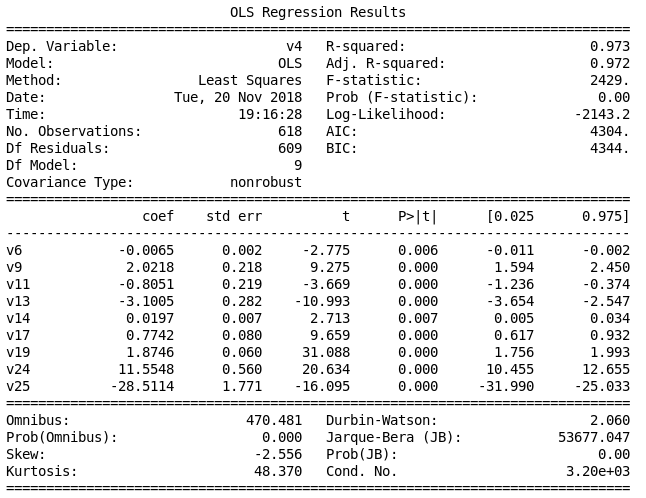
\includegraphics[scale=0.5]{v4_reg.png}
\begingroup
\captionof{figure}{Regression results for v4}
\endgroup

The regression experiments on \textit{v2} are shown in Table 3.\\


\begin{tabular}{|c|c|c|}
\hline 
\textbf{IVs} & \textbf{Adj. $R^2$} & \textbf{Significant IVs} \\ 
\hline 
v4 & 0.804 & All \\ 
\hline 
v4 (no const) & 0.818 & All \\ 
\hline 
v4,v6 & 0.924 & All \\ 
\hline 
v4,v6 (no const) & 0.93 & All \\ 
\hline 
v4,v6,v9 & 0.924 & All except constant \\ 
\hline 
v4,v6,v9 (no const) & 0.93 & All \\ 
\hline 
v4,v6,v9,v10 & 0.925 & All \\ 
\hline 
v4,v6,v9,v10 (no const) & 0.931 & All except v9 \\ 
\hline 
v4,v6,v9,v10,v14 & 0.933 & All \\ 
\hline 
v4,v6,v9,v10,v14 (no const) & 0.939 & All \\ 
\hline 
v4,v6,v9,v10,v14,v16 & 0.981 & All except constant  \\ 
\hline 
v4,v6,v9,v10,v14,v16 (no const) & 0.983 & All \\ 
\hline 
v4,v6,v9,v10,v14,v16,v18 & 0.981 & All except constant and v18 \\ 
\hline 
v4,v6,v9,v10,v14,v16,v18 (no const) & 0.983 & All except v18 \\ 
\hline 
v4,v6,v9,v10,v14,v16,v18,v19 & 0.992 & All \\ 
\hline 
\textbf{v4,v6,v9,v10,v14,v16,v18,v19 (no const)} & \textbf{0.993} & \textbf{All except v9} \\ 
\hline 
v4,v6,v9,v10,v14,v16,v18,v19,v24 & 0.992 & All \\ 
\hline 
v4,v6,v9,v10,v14,v16,v18,v19,v24 (no const) & 0.993 & All except v9 \\ 
\hline 
\end{tabular}

\begingroup
\captionof{table}{Regression experiments for v2}
\endgroup
\hfill\break
The chosen regression experiment is shown in Figure 2.
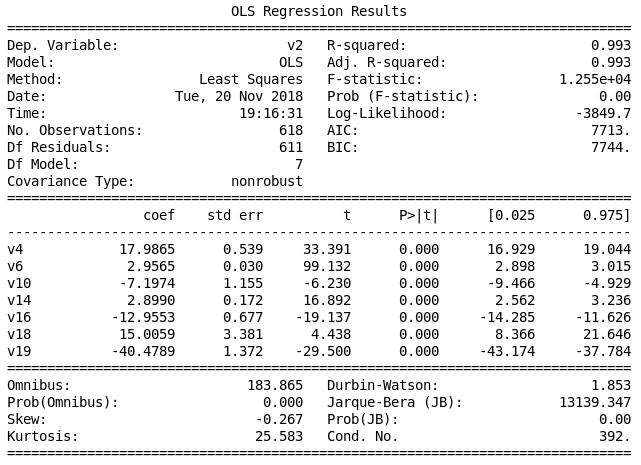
\includegraphics[scale=0.5]{v2_reg.png}
\begingroup
\captionof{figure}{Regression results for v2}
\endgroup
\hfill\break

From v6 onward, the experiments were automated. The screenshots of the program results are shown instead. The regression experiments for \textit{v6} are shown in Figure 3.
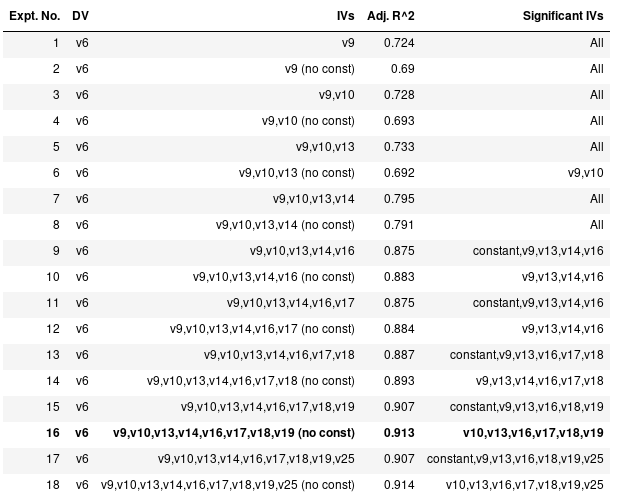
\includegraphics[scale=0.5]{v6_reg.png}
\begingroup
\captionof{figure}{Regression experiments for v6}
\endgroup

The chosen regression results are shown in Figure 4.\\

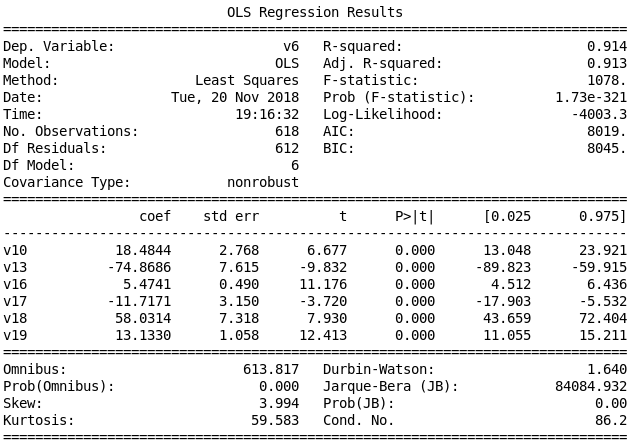
\includegraphics[scale=0.5]{v6_exp.png}
\begingroup
\captionof{figure}{Regression results for v6}
\endgroup

Figure 5 shows the regression experiments for \textit{v9}.\\

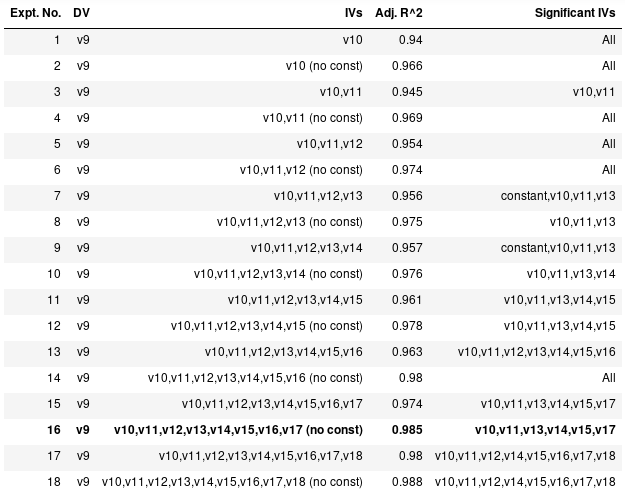
\includegraphics[scale=0.5]{v9_reg.png}
\begingroup
\captionof{figure}{Regression experiments for v9}
\endgroup

Figure 6 shows the chosen regression results.\\

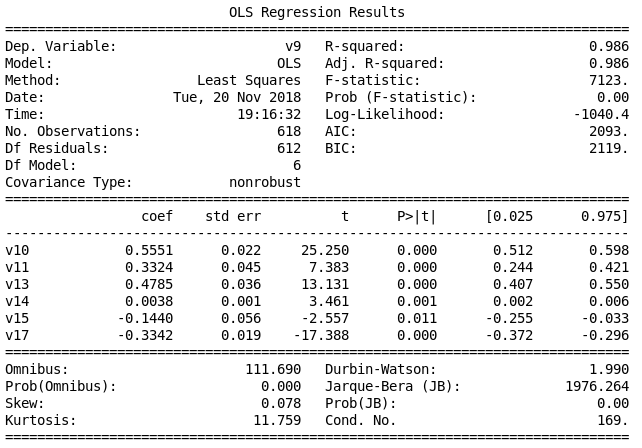
\includegraphics[scale=0.5]{v9_exp.png}
\begingroup
\captionof{figure}{Regression results for v9}
\endgroup
\hfill\break

The regression experiments for \textit{v10} are shown in Figure 7.

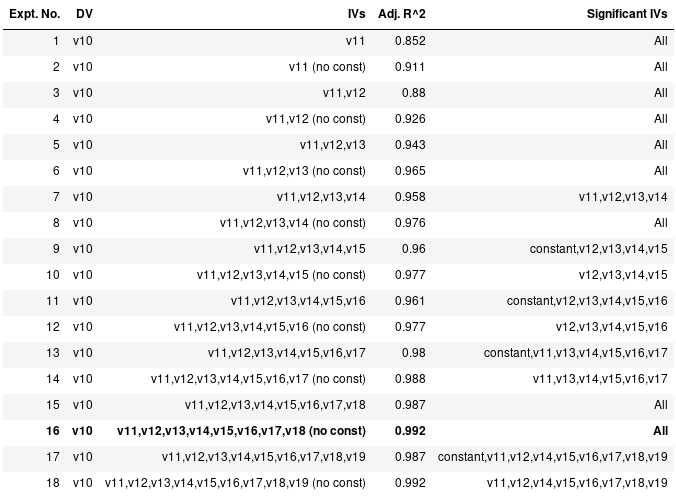
\includegraphics[scale=0.5]{v10_reg.png}
\begingroup
\captionof{figure}{Regression experiments for v10}
\endgroup

Finally, the results of the regression for \textit{v10} are shown in Figure 8.\\

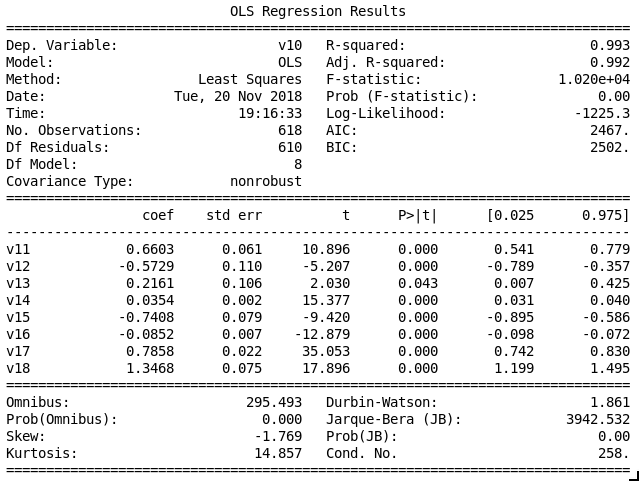
\includegraphics[scale=0.5]{v10_exp.png}
\begingroup
\captionof{figure}{Regression results for v10}
\endgroup

\subsection{Analysis on subset of data}
We now present the regression experiments and results on the chosen subset of the data. Please note that we renamed the variables for convenience, so \textit{v1} through \textit{v13} here are really \textit{v9} through \textit{v21}, and \textit{v14} here is really \textit{v24}.

The regression experiments for \textit{v9} (shown as \textit{v1}) are shown in Figure 9.\\

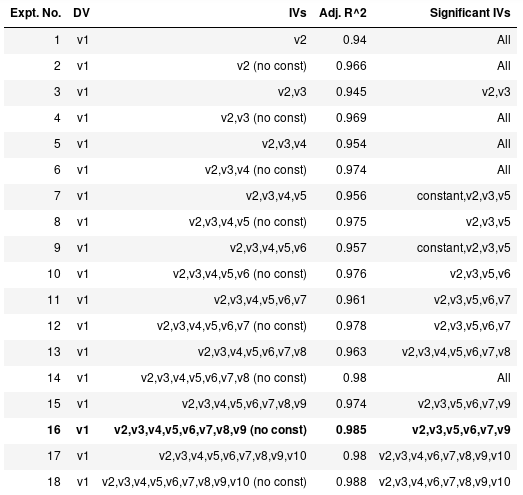
\includegraphics[scale=0.5]{v1_sub_reg.png}
\begingroup
\captionof{figure}{Regression experiments for v9}
\endgroup
\hfill\break

The chosen regression model results are shown in Figure 10.\\

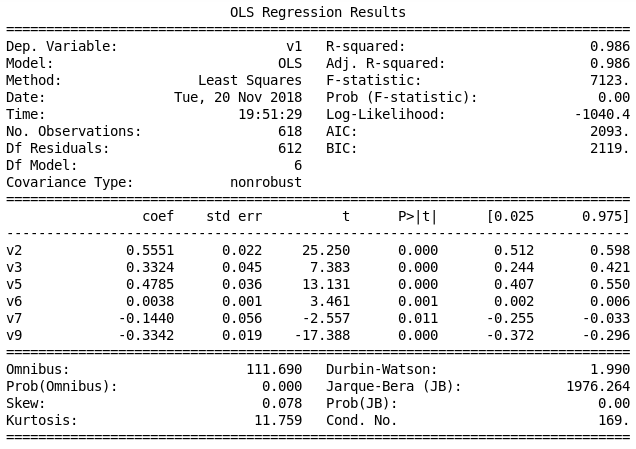
\includegraphics[scale=0.5]{v1_sub_exp.png}
\begingroup
\captionof{figure}{Regression results for v9}
\endgroup
\hfill\break

The regression experiments for \textit{v10} are shown in Figure 11.\\

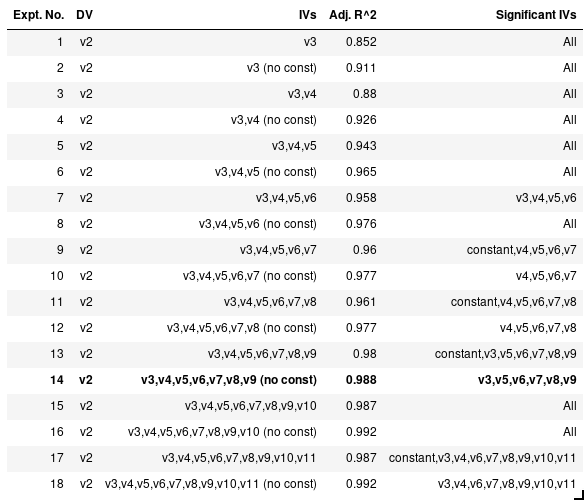
\includegraphics[scale=0.5]{v2_sub_reg.png}
\begingroup
\captionof{figure}{Regression experiments for v10}
\endgroup
\hfill\break

The chosen model for \textit{v10} is shown in Figure 12.\\

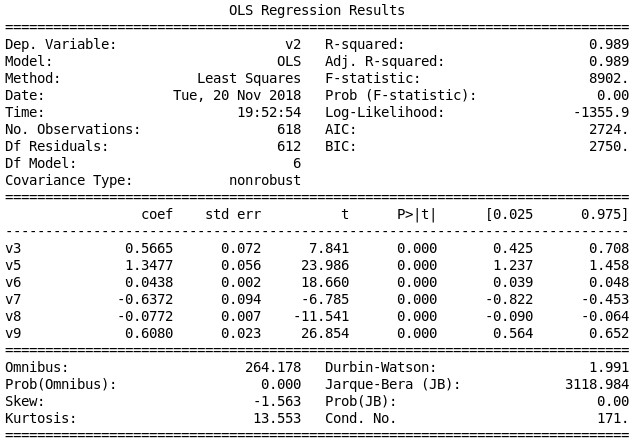
\includegraphics[scale=0.5]{v2_sub_exp.png}
\begingroup
\captionof{figure}{Regression results for v10}
\endgroup
\hfill\break

Next, we show Figure 13 and 14, which show the experiments and results for \textit{v11}.\\

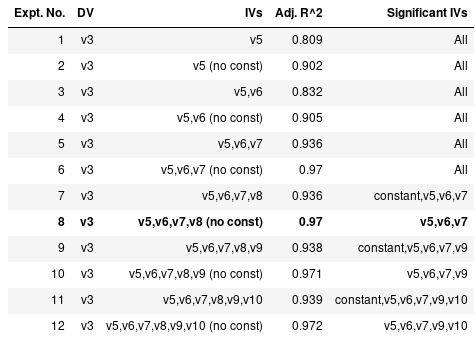
\includegraphics[scale=0.5]{v3_sub_reg.png}
\begingroup
\captionof{figure}{Regression experiments for v11}
\endgroup
\hfill\break

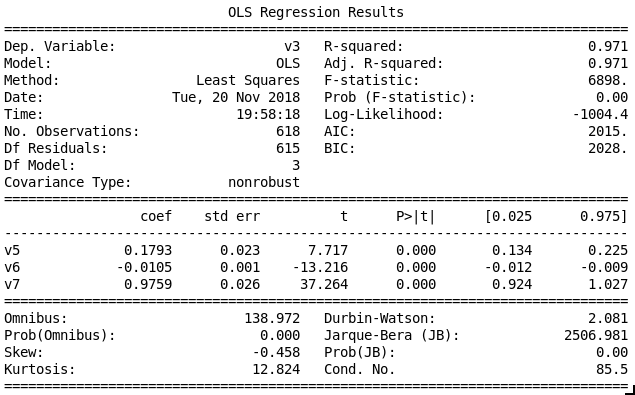
\includegraphics[scale=0.5]{v3_sub_exp.png}
\begingroup
\captionof{figure}{Regression results for v11}
\endgroup
\hfill\break

Finally(!), we show the same set of figures for \textit{v13}.\\

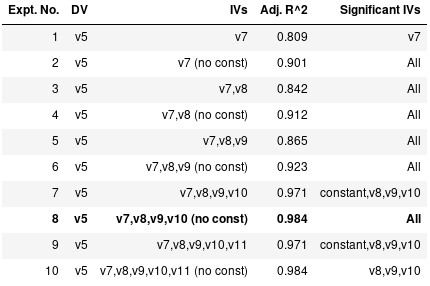
\includegraphics[scale=0.5]{v5_sub_reg.png}
\begingroup
\captionof{figure}{Regression experiments for v13}
\endgroup
\hfill\break

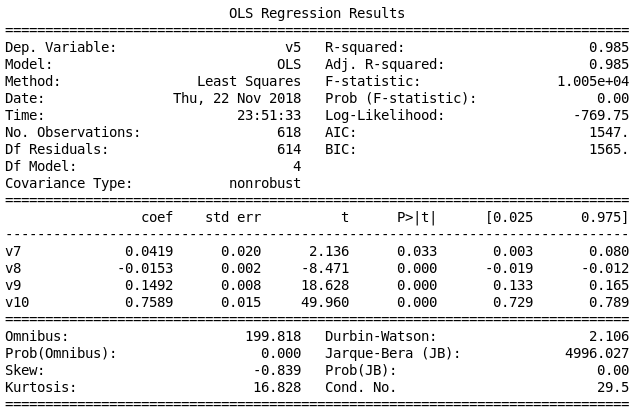
\includegraphics[scale=0.5]{v5_sub_exp.png}
\begingroup
\captionof{figure}{Regression results for v13}
\endgroup

\section{Cluster Analysis}
We now present the full description of where each point is in each clustering algorithm. The explanation in the paper supplements this well enough to clearly understand the segregation of points by both algorithms.

\subsection{PCA}
We performed a PCA before using DBSCAN. In all cases, we used the same method discussed in the paper to compute the value of \textit{eps}. We did this analysis for one through twelve dimensions. For number of dimensions greater than six, the performance stagnates at 0.571. We argue however, that the new dimensions obtained by PCA are less interpretable than simply using the original features, and the maximum difference between the performance of DBSCAN using our hand-picked features (0.571) and using PCA (0.644, n=2) was only 0.073. Figure 17 shows the results of using PCA to various numbers of dimensions.

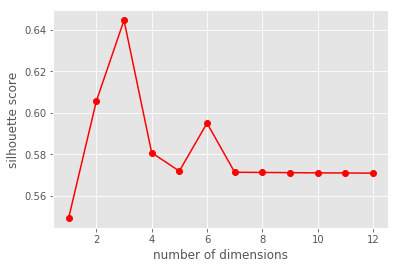
\includegraphics[scale=0.7]{pca.png}
\begingroup
\captionof{figure}{Results of using PCA and then clustering with DBSCAN}
\endgroup

\subsection{Analysis on $S_1$}
Figure 18 shows the analysis for $S_1$. The Silhouette score for DBSCAN here was 0.635.

We make the following observations. The largest clusters for both the algorithms are very similar \textbf{(row 9)}. The two points in the MS cluster that were not in DBSCAN's largest cluster were in its second largest cluster \textbf{(row 2)}. All the clusters of the mean-shift algorithm that were of size 4 or less were marked as individual clusters by DBSCAN \textbf{(rows 5-8 and row 1)}. More surprisingly, the cluster of 19 points identified by mean-shift was marked as 19 individual clusters by DBSCAN \textbf{(row 4)}. Finally, a considerable part of mean-shift's second-largest cluster was also identified as individual points by DBSCAN \textbf{(row 3)}.

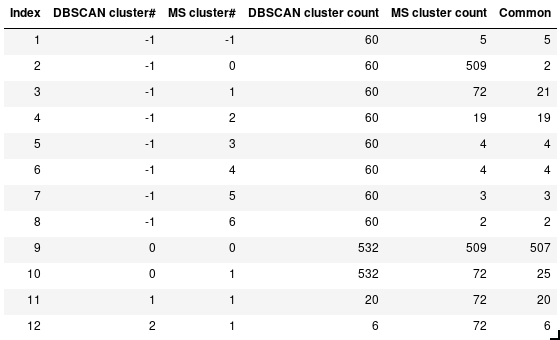
\includegraphics[scale=0.65]{cluster_s1.png}
\begingroup
\captionof{figure}{Clustering by DBSCAN and Mean-Shift algorithms on $S_1$}
\endgroup

\subsection{Analysis on $S_2$}
Figure 19 shows the analysis for $S_2$. As noted in the paper, the Silhouette score for DBSCAN for this subset was 0.571. \\

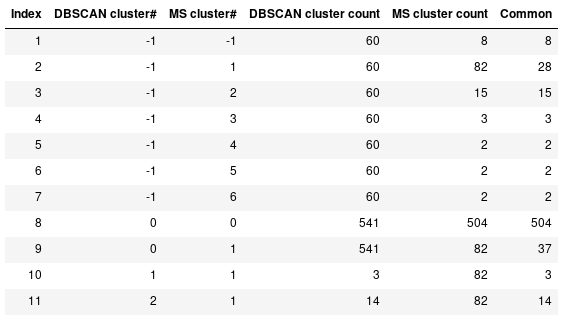
\includegraphics[scale=0.65]{clustering.png}
\begingroup
\captionof{figure}{Clustering by DBSCAN and Mean-Shift algorithms on $S_2$}
\endgroup

\end{document}